\documentclass[geye,green,pad,en]{elegantnote}

\title{ElegantNote: An Elegant \LaTeX{} Template for Notes}

\author{\href{https://ddswhu.me/}{Dongsheng Deng}}
\institute{\href{https://elegantlatex.org/}{Elegant\LaTeX{} Program}}
\version{2.20}

\date{\today}

\begin{document}
\maketitle
% logo
\centerline{
\includegraphics[width=0.25\textwidth]{logo.pdf}}

\section{Features Overview}
This template was originally designed to take notes and was conceived in 2013. In the first version, we designed a  series of beautiful theorem environments and introduced 3 different color themes. But when taking notes using this template, we found there were so many theorem blocks which makes the notes not pretty. So we decided to update the ElegantNote to the ElegantBook template. The design of ElegantNote stopped there.

In 2018, after being "urged" by some users, ElegantBook received a major update, the original floating theorem environments are rewritten with tcolorbox package. After that, we want to completely redesign the ElegantNote template. We are in favor of more compact, simpler theorem environments, and aim to design an Elegant \LaTeX{} template which is more suitable for note taking and note reading.

With the advice and inspiration of some friends, we redesigned the new ElegantNote template based on the Standard \LaTeX{} article class! The new template has the following features:

\begin{itemize}
\item good for eye mode: with green page color;
\item different devices: Pad (default), Kindle, PC (double-page) and normal (A4);
\item 5 color themes: \textcolor{egreen}{green} (default), \textcolor{ecyan}{cyan}, \textcolor{eblue}{blue}, \textcolor{sakura}{sakura}, \textcolor{black}{black};
\item languages support: Chinese (default), English;
\item support \lstinline{PDFLaTeX} and \lstinline{XeLaTeX};
\item prettier captions, list environments, and unified fonts.
\end{itemize}

\subsection{Good for Eye Mode}
This template added good for eye mode (geye), the default is none, you can switch to good eye mode using:
\begin{lstlisting}[frame=none]  
\documentclass[geye]{elegantnote}  % or
\documentclass[mode=geye]{elegantnote}
\end{lstlisting}

\begin{remark}
In this version, only one background color is added. If you are expected to add other colors, you can create issues or pull requests at \href{https://github.com/ElegantLaTeX/ElegantNote}{Github/ElegantNote}.
\end{remark}

\subsection{Device Options}

To make the notes more comfortable to read, we designed four output options (of different sizes) that correspond to different reading devices: Pad, Kindle, PC and A4paper. The options of output for different devices are
\begin{lstlisting}[frame=none]  
\documentclass[device=pad]{elegantnote}
\documentclass[device=kindle]{elegantnote}
\documentclass[device=pc]{elegantnote}
\documentclass[device=normal]{elegantnote}
\end{lstlisting}
\begin{note}
You can also select the device by using a direct assignment method, such as:
\end{note}
\begin{lstlisting}[frame=none]  
\documentclass[pad]{elegantnote}
\documentclass[kindle]{elegantnote}
\documentclass[pc]{elegantnote}
\documentclass[normal]{elegantnote}
\end{lstlisting}

\begin{note}
Note that if you want a normal A4paper size PDF, you need to select \lstinline{device=normal} instead of \lstinline{device=pc} , because \lstinline{device=pc} is actually set to double page mode on your computer.
\end{note}
\subsection{Color Themes}
This template contains 5 color themes, \textcolor{egreen}{green}, \textcolor{ecyan}{cyan}, \textcolor{eblue}{blue}, \textcolor{sakura}{sakura}, \textcolor{black}{black}. Where green is the default color theme, if you don't need color, you can choose black theme. The color theme is enabled in the same way as before:
\begin{lstlisting}[frame=none]  
\documentclass[green]{elegantnote}
\documentclass[color=green]{elegantnote}
....
\documentclass[black]{elegantnote}
\documentclass[color=black]{elegantnote}
\end{lstlisting}

\subsection{Languages}
This template contains two sets of language environments, changing the language environment will change the title of table/figure (figure, table), article structure words (such as the table of contents, references, etc.), and the environment Introductory words (such as Theorem, Lemma, etc.). The different language modes are enabled as follows:
\begin{lstlisting}[frame=none]  
\documentclass[cn]{elegantnote}
\documentclass[lang=cn]{elegantnote}
\documentclass[en]{elegantnote}
\documentclass[lang=en]{elegantnote}
\end{lstlisting}
\begin{note}
You can input Chinese Character in \lstinline{lang=en} mode only.
\end{note}

\subsection{Compilation Methods}

You can use \lstinline{PDFLaTeX} or \lstinline{XeLaTeX} to process your notes. If you are using \lstinline{PDFLaTeX}, \lstinline{ctex} package is used, and if you are using \lstinline{XeLaTeX}, \lstinline{ctex} package is called when processing Chinese characters. 

The test environment is Win10 + \TeX{} Live 2018. If you are using a Mac/Linux system and compiled with \lstinline{XeLaTeX},  please change the font in \lstinline{elegantnote.cls} with your system font.

\begin{note}
If you are using \lstinline{PDFLaTeX}, you do not need to change the font settings.
\end{note}

\subsection{Theorem Class Environments}
This template used the \lstinline{amsthm} to create theorems, there are 4 types of theorem environments
\begin{itemize}
\item \textbf{Theorem-Class}: theorem, lemma, proposition, corollary;
\item \textbf{Definition-Class}: definition, conjecture, example;
\item \textbf{Remark-Class}: remark, note, case;
\item \textbf{Proof-Class}: proof.
\end{itemize}

\begin{remark}
With the option \lstinline{lang=cn} , the introductory words of the theorem class environments will be changed to Chinese.
\end{remark}

\section{Writing Sample}

We will define the integral of a measurable function in three steps. First, we define the integral of a nonnegative simple function. Let $E$ be the measurable set in $\mathcal{R}^N$.

% source: https://www.maths.tcd.ie/~dwilkins/LaTeXPrimer/Theorems.html

\begin{definition}[Left Coset]
Let $H$ be a subgroup of a group~$G$.  A \emph{left coset} of $H$ in $G$ is a subset of $G$ that is of the form $xH$, where $x \in G$ and $xH = \{ xh : h \in H \}$. Similarly a \emph{right coset} of $H$ in $G$ is a subset of $G$ that is of the form $Hx$, where $Hx = \{ hx : h \in H \}$
\end{definition}

Note that a subgroup~$H$ of a group $G$ is itself a left coset of $H$ in $G$.

\begin{lemma}[Size Of Left Coset]
Let $H$ be a finite subgroup of a group $G$.  Then each left
coset of $H$ in $G$ has the same number of elements as $H$.
\end{lemma}

\begin{theorem}[Lagrange's Theorem]
Let $G$ be a finite group, and let $H$ be a subgroup
of $G$.  Then the order of $H$ divides the order of $G$.
\end{theorem}

\begin{proof}
Let $z$ be some element of $xH \cap yH$.  Then $z = xa$ for some $a \in H$, and $z = yb$ for some $b \in H$. If $h$ is any element of $H$ then $ah \in H$ and $a^{-1}h \in H$, since $H$ is a subgroup of $G$. But $zh = x(ah)$ and $xh = z(a^{-1}h)$ for all $h \in H$. Therefore $zH \subset xH$ and $xH \subset zH$, and thus $xH = zH$.  Similarly $yH = zH$, and thus $xH = yH$, as required.
\end{proof}

\begin{figure}[!htbp]
	\centering
	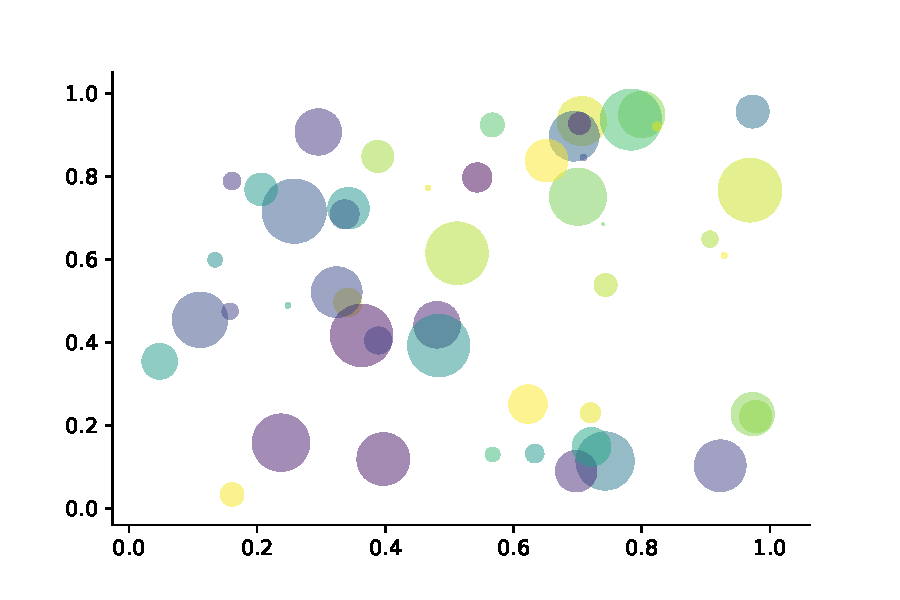
\includegraphics[width=0.6\textwidth]{scatter.pdf}
	\caption{Matplotlib: Scatter Plot Example\label{fig:mpg}}
\end{figure}

Regression analysis is a powerful statistical method that allows you to examine the relationship between two or more variables of interest. While there are many types of regression analysis, at their core they all examine the influence of one or more independent variables on a dependent variable. The process of performing a regression allows you to confidently determine which factors matter most, which factors can be ignored, and how these factors influence each other.

Let's continue using our application training example. In this case, we'd want to measure the historical levels of satisfaction with the events from the past three years or so, as well as any information possible in regards to the independent variables. 


\begin{table}[htbp]
  \small
  \centering
  \caption{Auto MPG and Price \label{tab:reg}}
    \begin{tabular}{lcc}
    \toprule
                    &       (1)         &        (2)      \\
    \midrule
    mpg             &    -238.90***     &      -49.51     \\
                    &     (53.08)       &      (86.16)    \\
    weight          &                   &      1.75***    \\
                    &                   &      (0.641)    \\
    constant        &     11,253***     &       1,946     \\
                    &     (1,171)       &      (3,597)   \\
    obs             &        74         &         74     \\
    $R^2$           &      0.220        &       0.293    \\
    \bottomrule
    \multicolumn{3}{l}{\scriptsize Standard errors in parentheses} \\
    \multicolumn{3}{l}{\scriptsize *** p<0.01, ** p<0.05, * p<0.1} \\
    \end{tabular}%
\end{table}%


\begin{itemize}[noitemsep]
	\item Routing and resource discovery;
	     \begin{itemize} 
      	   	\item Language Models
       	 	\item Vector Space Models
    		 \end{itemize}
	\item Resilient and scalable computer networks;
	\item Distributed storage and search.
\end{itemize}

\section{A Minimal Example}
\begin{lstlisting}[frame=single]  
\documentclass[geye,green,pad,en]{elegantnote}

\title{A Note Example}

\author{ddswhu}
\institute{Elegant\LaTeX{} Program}
\version{1.00}
\date{\today}

\begin{document}

\maketitle

\section{Introduction}
Example Text.

\end{document}
\end{lstlisting}
\end{document}
